\documentclass{beamer}
\usetheme{Madrid}
\usecolortheme{default}

% Packages
\usepackage{graphicx}
\usepackage{booktabs}
\usepackage{amsmath}
\usepackage{amsfonts}
\usepackage{tabularx}

% Metadata
\title[Cracked Egg Detection]{\large \textbf{REAL-TIME DETECTION METHOD FOR CRACKED EGGS BASED ON IMPROVED YOLOV8 AND DUAL VERIFICATION WITH TRIPLE CLASSIFICATION GRANULARITY}}
\subtitle{CSQ413 Seminar Presentation}

\author[Arjun Manoj | CEC23CS043]{
\textbf{Submitted by:} \\ ARJUN MANOJ (CEC23CS043) \\[0.25cm]
\textbf{Under the Guidance of:} \\ Mrs. NANDANA RAJ R \\ Assistant Professor
}

\institute[]{
Department of Computer Science and Engineering \\ College of Engineering, Cherthala
}

\date{}

\begin{document}

% ==================== SLIDE 1: TITLE SLIDE ====================
\begin{frame}
  \titlepage
\end{frame}

% ==================== SLIDE 2: OUTLINE ====================
\begin{frame}{Outline}
\tableofcontents
\end{frame}

%=====================================================
\section{Introduction and Problem Statement}
%=====================================================

% ==================== SLIDE 3: INTRODUCTION ====================
\begin{frame}{Introduction}
\small
\begin{itemize}
    \item \textbf{Commercial Significance:} Eggshell integrity is a vital quality indicator in the poultry industry.
    \medskip
    \item \textbf{High Breakage Rate:} Around 3\% of eggs suffer shell damage during production, packing and transit.
    \medskip
    \item \textbf{Financial and Health Risks:} Cracks cause bacterial invasion, rapid spoilage, yolk leakage and financial losses.
    \medskip
    \item \textbf{Current Industry Reliance:} Still primarily rely on manual visual inspection.
    \medskip
    \item \textbf{Manual Bottlenecks:} Labor-intensive, low efficiency and prone to missed defects from worker fatigue.
\end{itemize}
\end{frame}

% ==================== SLIDE 4: LIMITATIONS OF EXISTING METHODS ====================
\begin{frame}{Limitations of Existing Methods}
\small
\begin{itemize}
    \item \textbf{Acoustic Resonance Methods:}
    \begin{itemize}
        \item Analyzes acoustic response from mechanical tapping.
        \item Vulnerable to severe ambient noise on factory floors; high equipment cost.
    \end{itemize}
    \medskip
    \item \textbf{Traditional Computer Vision:}
    \begin{itemize}
        \item Employs manual feature extraction (Otsu thresholding, morphological filters).
        \item Slow processing speed; fragile under fluctuating factory illumination.
    \end{itemize}
    \medskip
    \item \textbf{Existing Deep Learning Approaches:}
    \begin{itemize}
        \item High computational complexity; inference speeds struggle to sustain $\ge 30$ FPS.
        \item Evaluated primarily on static, pre-washed egg images.
        \item Absence of egg rotation creates uninspected blind spots on the bottom shell.
    \end{itemize}
\end{itemize}
\end{frame}

% ==================== SLIDE 5: RESEARCH OBJECTIVES ====================
\begin{frame}{Research Objectives and Key Contributions}
\small
\textbf{Primary Objective:} Develop an industrial-grade, real-time online detection method for unwashed cracked eggs on dynamic production lines.

\bigskip
\textbf{Core Contributions of the Study:}
\begin{itemize}
    \item \textbf{Triple Granularity and Dual Verification:} Classifies intact eggs, cracked eggs and crack regions with a joint decision rule to eliminate missed defects.
    \medskip
    \item \textbf{Structural YOLOv8 Optimization:} Embeds DCNv2, BiFPN, WIoUv2 loss and an extra small object head to capture subtle hairline cracks.
    \medskip
    \item \textbf{Live Industrial Deployment:} Deployed on a Kyowa/FP-600 egg conveyor with rotating rollers, achieving 45 FPS and meeting industrial reliability standards.
\end{itemize}
\end{frame}

%=====================================================
\section{Literature Survey}
%=====================================================

% ==================== SLIDE 6: LITERATURE SURVEY PART 1 ====================
\begin{frame}[t]{Literature Survey: Traditional and Two-Stage Methods}
\vspace{-0.2cm}
\begin{table}[t]
\centering
\caption{\scriptsize Literature survey of traditional image processing and two-stage deep learning methods}
\vspace{-0.3cm}
\setlength{\arrayrulewidth}{0.8pt}
\renewcommand{\arraystretch}{1.25}
\resizebox{\textwidth}{!}{
\begin{tabular}{>{\centering\arraybackslash}p{3.2cm} >{\centering\arraybackslash}p{2.8cm} >{\centering\arraybackslash}p{2.2cm} >{\centering\arraybackslash}p{2.0cm} >{\centering\arraybackslash}p{3.6cm}}
\hline
\textbf{Paper, Author, Year} & \textbf{Methodology} & \textbf{Dataset} & \textbf{Result} & \textbf{Limitations} \\
\hline
Integrated egg quality system \newline \textit{Liang et al. (2020)} & Histogram thresholding + Otsu segmentation & Static egg images (lab setup) & 98.18\% accuracy & Manual feature extraction; sensitive to lighting; static only. \\
\hline
Damage detection on eggshells \newline \textit{Datta et al. (2019)} & Faster R-CNN (two-stage detector) & Chicken eggshells (static) & 75\% mAP (severe cracks) & High computational complexity; inference too slow for real-time lines. \\
\hline
Defective egg detection via CNN-BiLSTM \newline \textit{Turkoglu (2021)} & Hybrid CNN-BiLSTM deep network & Egg surface defect dataset & 96.3\% accuracy & Heavy network architecture; serial processing limits line throughput. \\
\hline
\end{tabular}
}
\end{table}
\end{frame}

% ==================== SLIDE 7: LITERATURE SURVEY PART 2 ====================
\begin{frame}[t]{Literature Survey: Deep Learning and YOLO Adaptations}
\vspace{-0.2cm}
\begin{table}[t]
\centering
\caption{\scriptsize Literature survey of convolutional and YOLO-based egg crack inspection methods}
\vspace{-0.3cm}
\setlength{\arrayrulewidth}{0.8pt}
\renewcommand{\arraystretch}{1.25}
\resizebox{\textwidth}{!}{
\begin{tabular}{>{\centering\arraybackslash}p{3.2cm} >{\centering\arraybackslash}p{2.8cm} >{\centering\arraybackslash}p{2.2cm} >{\centering\arraybackslash}p{2.0cm} >{\centering\arraybackslash}p{3.6cm}}
\hline
\textbf{Paper, Author, Year} & \textbf{Methodology} & \textbf{Dataset} & \textbf{Result} & \textbf{Limitations} \\
\hline
Eggshell crack detection \newline \textit{Botta et al. (2022)} & Deep Convolutional Neural Networks & Static chicken egg images & 95.38\% accuracy & Optimized only for static scenes; misses bottom cracks due to lack of rotation. \\
\hline
Lightweight duck egg crack detection \newline \textit{Yin et al. (2024)} & YOLOv5 + Ghost modules + ECA attention & Cracked duck egg dataset & 93.8\% accuracy & Tested only on duck eggs; binary labeling misses subtle hairline cracks. \\
\hline
Damage detection of unwashed eggs \newline \textit{Huang et al. (2023)} & YOLOv5 + BiFPN + GSConv + CA attention & Dynamic video of unwashed eggs & 96.4\% accuracy & Lacks dual verification of localized crack regions; bottom cracks uninspected. \\
\hline
\end{tabular}
}
\end{table}
\end{frame}

%=====================================================
\section{System Hardware and Data Acquisition}
%=====================================================

% ==================== SLIDE 8: SYSTEM HARDWARE ====================
\begin{frame}{System Hardware and Conveying Mechanism}
\small
\begin{itemize}
    \item \textbf{Multi-Channel Conveyor:} 6 parallel channels carrying 60 eggs/min each (total throughput: 360 eggs/min).
    \medskip
    \item \textbf{Compound Motion (Translation + Rotation):} Motor-driven rollers rotate eggs 360 degrees, presenting all shell surfaces to the camera.
    \medskip
    \item \textbf{Parallel Camera Alignment:} CCD camera imaging plane is positioned parallel to egg motion plane to prevent perspective distortion.
    \medskip
    \item \textbf{Regulated Lighting:} Integrated LED illumination box ensures uniform brightness across all channels.
\end{itemize}
\end{frame}

% ==================== SLIDE 9: FULL SLIDE FIGURES 1 & 2 ====================
\begin{frame}{Conveying Device and Vision System Setup}
\begin{figure}[h]
    \centering
    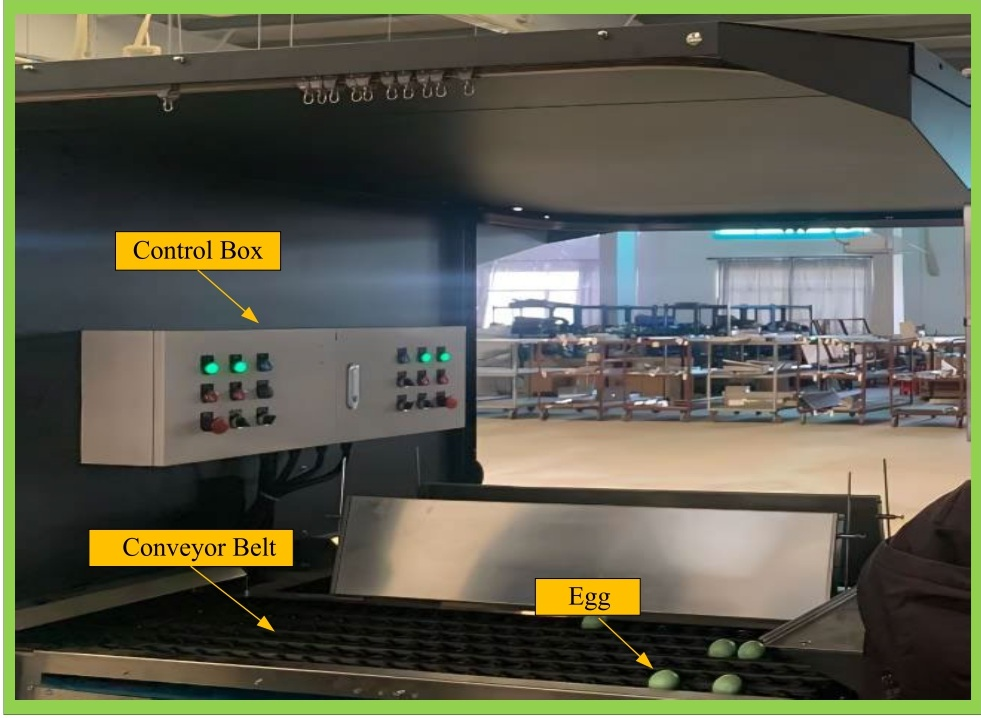
\includegraphics[width=0.48\linewidth,height=0.72\textheight,keepaspectratio]{figure1_egg_conveying_device.jpg}
    \hfill
    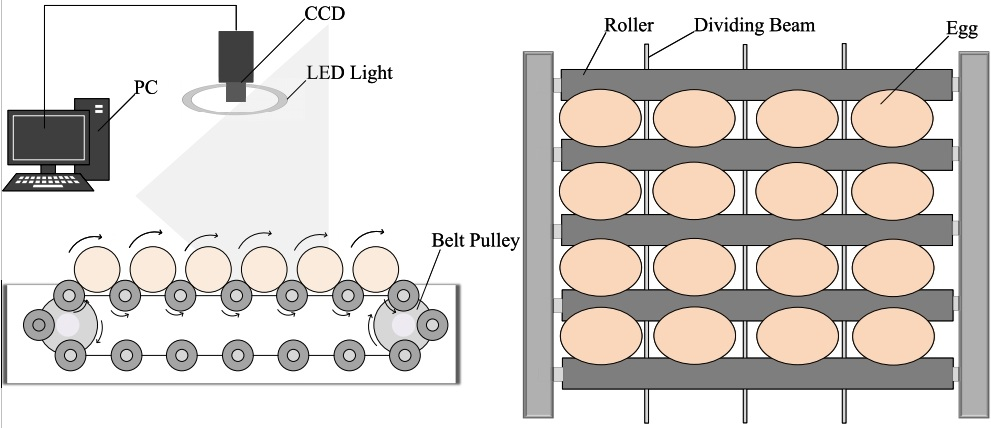
\includegraphics[width=0.48\linewidth,height=0.72\textheight,keepaspectratio]{figure2_machine_vision_system.jpg}
    \vspace{-0.2cm}
    \caption{\scriptsize Left: Egg conveying device with 6 channels (Figure 1). Right: Machine vision system schematic (Figure 2).}
\end{figure}
\end{frame}

% ==================== SLIDE 10: DATASET ACQUISITION ====================
\begin{frame}{Dataset Acquisition and Preparation}
\small
\begin{itemize}
    \item \textbf{Industrial Collection:} Captured on live conveyor at Guangzhou Suiping Enterprise Co., Ltd.
    \medskip
    \item \textbf{Real-World Conditions:} Tested on unwashed eggs with dust, stains and factory lighting variations.
    \medskip
    \item \textbf{Balanced Sampling:} 628 raw dynamic images with deliberate inclusion of cracked eggs.
    \medskip
    \item \textbf{Data Augmentation:} Random cropping and flipping (50\% probability) expanded training set to 2,972 images.
    \medskip
    \item \textbf{Final Dataset (6:2:2 Split):} 3,222 total images containing 7,611 intact eggs, 2,711 cracked eggs and 2,935 cracked areas.
\end{itemize}
\end{frame}

% ==================== SLIDE 11: TRIPLE GRANULARITY ====================
\begin{frame}{Triple Classification Granularity}
\begin{itemize}
    \item \textbf{Category 1 (Intact Egg):} Normal undamaged egg body.
    \item \textbf{Category 2 (Cracked Egg):} Entire egg body displaying cracks.
    \item \textbf{Category 3 (Crack Region):} Specific localized micro-damage zone.
\end{itemize}
\vspace{-0.1cm}
\begin{figure}[h]
    \centering
    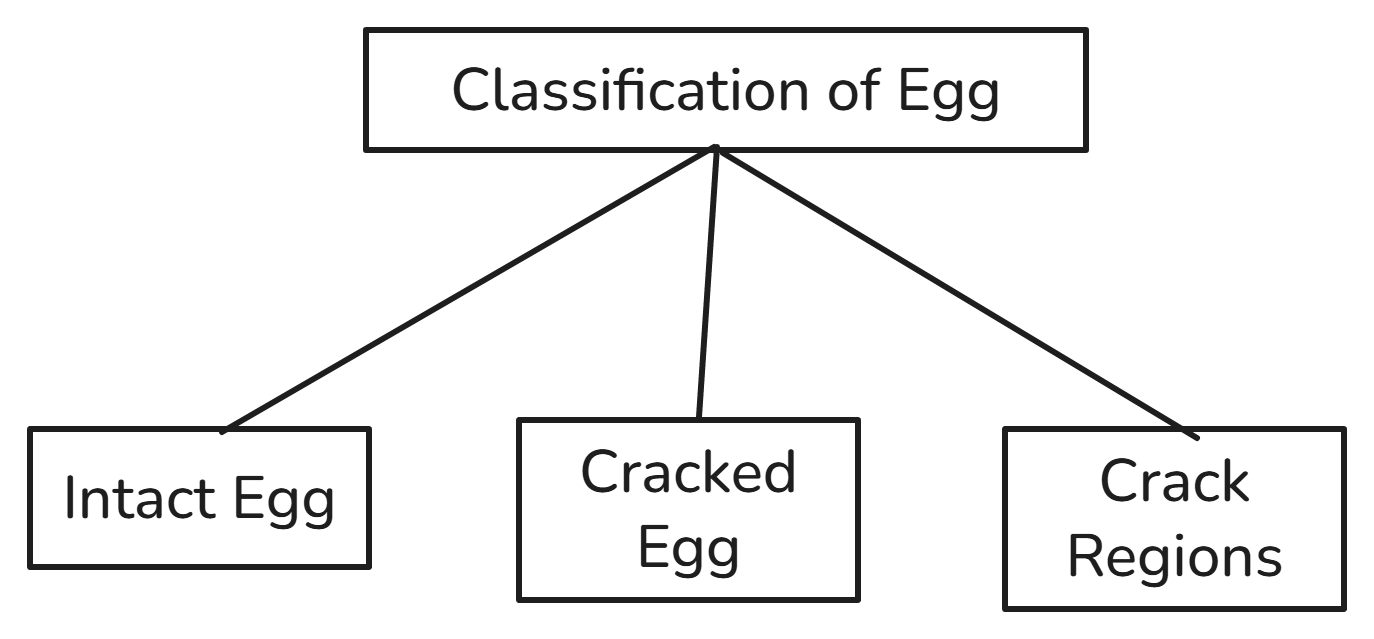
\includegraphics[width=0.92\linewidth,height=0.52\textheight,keepaspectratio]{classificationCategories.png}
    \vspace{-0.2cm}
    \caption{\scriptsize Classification categories: Intact eggs, cracked eggs and localized crack regions.}
\end{figure}
\end{frame}

%=====================================================
\section{Proposed Improved YOLOv8 Methodology}
%=====================================================

% ==================== SLIDE 12: ARCHITECTURE OVERVIEW (MAIN PIPELINE) ====================
\begin{frame}{Improved YOLOv8 Network Architecture: Main Pipeline}
\begin{figure}[h]
    \centering
    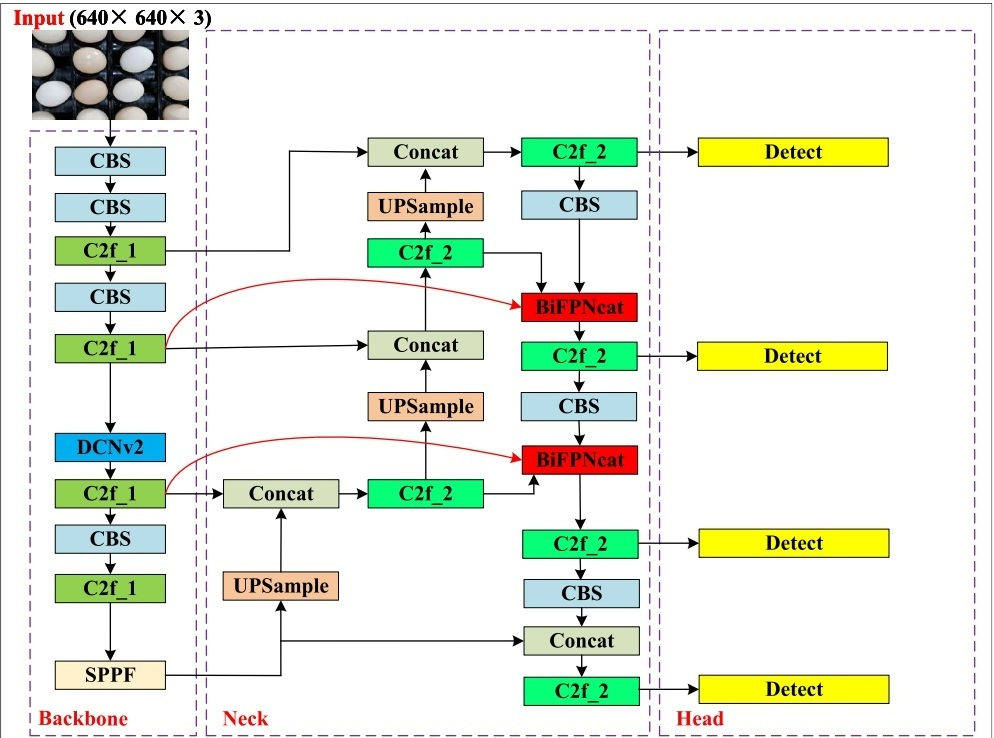
\includegraphics[width=0.95\linewidth,height=0.78\textheight,keepaspectratio]{figure3_improved_yolov8_architecture_1.jpg}
    \vspace{-0.2cm}
    \caption{\scriptsize Improved YOLOv8 overall detection architecture (Source: Base Paper Figure 3).}
\end{figure}
\end{frame}

% ==================== SLIDE 13: ARCHITECTURAL SUB-MODULES ====================
\begin{frame}{Improved YOLOv8: Structural Sub-Module Details}
\begin{figure}[h]
    \centering
    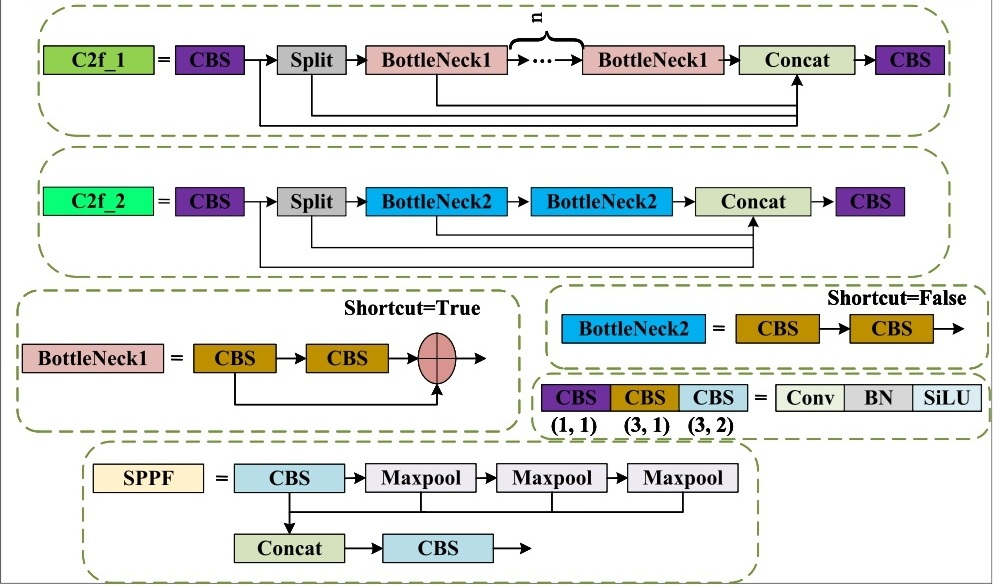
\includegraphics[width=0.95\linewidth,height=0.78\textheight,keepaspectratio]{figure3_improved_yolov8_architecture_2.jpg}
    \vspace{-0.2cm}
    \caption{\scriptsize Detailed network sub-module structures: C2f, BottleNeck and SPPF (Source: Base Paper Figure 3).}
\end{figure}
\end{frame}

% ==================== SLIDE 13: DCNv2 ====================
\begin{frame}{Architectural Enhancement 1: Deformable Convolutions (DCNv2)}
\begin{itemize}
    \item \textbf{Motivation:} Standard square kernels cannot conform to irregular, jagged crack geometry.
    \item \textbf{Mechanism:} DCNv2 adds learnable spatial offsets and dynamic modulation scalars to adapt receptive fields.
\end{itemize}
\vspace{-0.15cm}
\begin{equation*}
Y(q) = \sum_{k=1}^{K} w_k X(q + q_k + \Delta q_k) \Delta m_k
\end{equation*}
\vspace{-0.25cm}
\textbf{Symbol Definitions:}
\vspace{0.12cm}
\begin{itemize}
    \item $X, Y$: Input and output feature maps.
    \item $q$: Center target coordinate; $q_k$: Predefined grid offset ($k=1,\dots,K$).
    \item $w_k$: Convolutional kernel weight for the $k$-th location.
    \item $\Delta q_k$: Learnable 2D spatial offset adapting to geometric crack contours.
    \item $\Delta m_k$: Learnable modulation scalar ($\Delta m_k \in [0, 1]$) scaling feature amplitude.
\end{itemize}
\end{frame}

% ==================== SLIDE 14: DCNv2 SAMPLING (FULL SLIDE FIGURE 4) ====================
\begin{frame}{DCNv2: Sampling Strategy Comparison}
\begin{figure}[h]
    \centering
    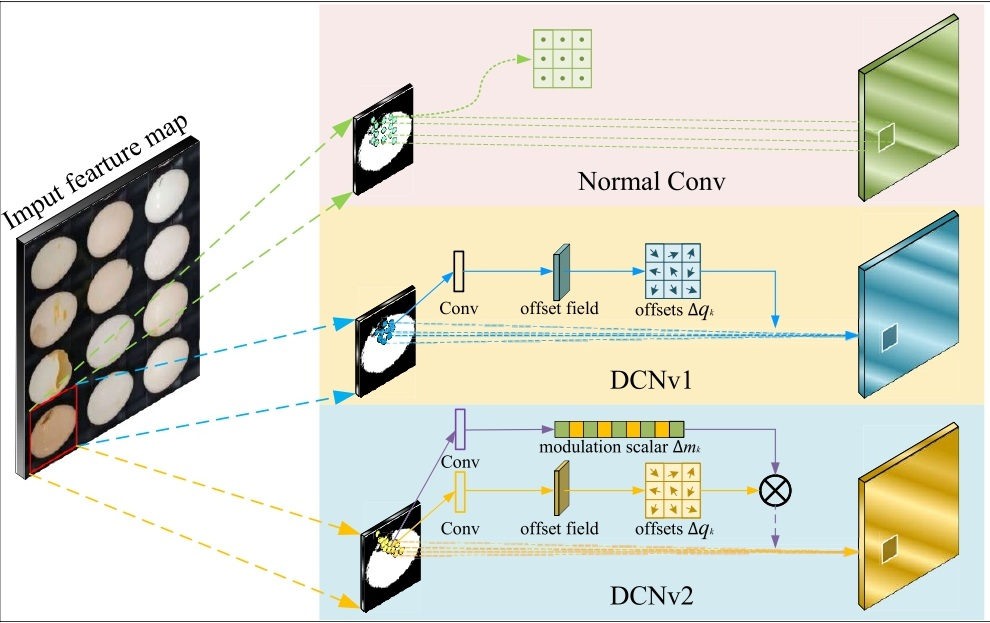
\includegraphics[width=0.88\linewidth,height=0.75\textheight,keepaspectratio]{figure4_dcnv2_sampling_comparison.jpg}
    \vspace{-0.2cm}
    \caption{\scriptsize Sampling comparison of Normal Conv, DCNv1 and DCNv2 (Source: Base Paper Figure 4).}
\end{figure}
\end{frame}

% ==================== SLIDE 15: BiFPN ====================
\begin{frame}{Architectural Enhancement 2: BiFPN Multi-Scale Fusion}
\small
\begin{itemize}
    \item \textbf{FPN vs PANet vs BiFPN Evolution:}
    \begin{itemize}
        \item \textbf{FPN:} Top-down pathway conveying high-level semantics.
        \item \textbf{PANet (Default YOLOv8):} Adds a bottom-up path for low-level spatial details.
        \item \textbf{BiFPN:} Removes single-edge nodes, adds cross-scale residual skips and repeats blocks.
    \end{itemize}
    \medskip
    \item \textbf{Weighted Feature Fusion:} Assigns learnable weights to different scale features based on importance.
    \medskip
    \item \textbf{Environmental Robustness:} Retains subtle crack cues despite factory lighting changes and shell dirt.
\end{itemize}
\end{frame}

% ==================== SLIDE 16: BiFPN STRUCTURE (FULL SLIDE FIGURE 5) ====================
\begin{frame}{Feature Pyramid Architectures: FPN, PANet and BiFPN}
\begin{figure}[h]
    \centering
    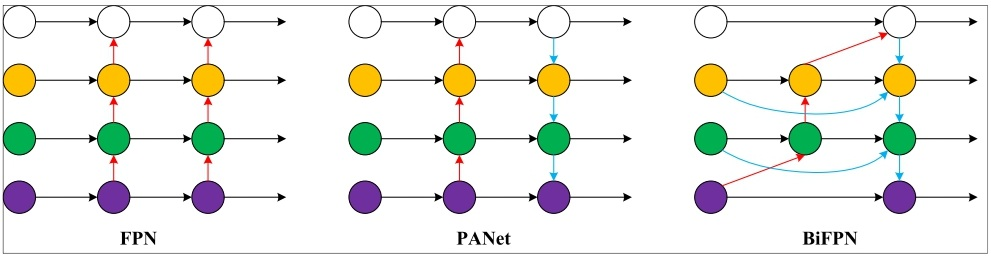
\includegraphics[width=0.9\linewidth,height=0.75\textheight,keepaspectratio]{figure5_fpn_panet_bifpn_structure.jpg}
    \vspace{-0.2cm}
    \caption{\scriptsize Structural comparison of FPN, PANet and BiFPN (Source: Base Paper Figure 5).}
\end{figure}
\end{frame}

% ==================== SLIDE 17: SMALL OBJECT HEAD AND WIoUv2 ====================
\begin{frame}{Enhancements 3 \& 4: Small Target Head and WIoUv2 Loss}
\begin{itemize}
    \item \textbf{Small Target Detection Head (P2 Layer):}
    \begin{itemize}
        \item Default YOLOv8 downsamples 5 times ($/32$); smallest head ($80 \times 80$) misses sub-8 px cracks.
        \item Added a 4th head on $160 \times 160$ feature map, directly utilizing early spatial details.
    \end{itemize}
    \item \textbf{Wise-IoU v2 (WIoUv2) Loss Function:}
\end{itemize}
\vspace{-0.15cm}
\begin{equation*}
L_{\text{WIoUv2}} = L_{\text{IoU}}^{\gamma*} L_{\text{WIoUv1}}, \quad \gamma > 0
\end{equation*}
\vspace{-0.25cm}
\textbf{Symbol Definitions:}
\vspace{0.12cm}
\begin{itemize}
    \item $L_{\text{WIoUv2}}$: Final Wise-IoU v2 bounding box regression loss.
    \item $L_{\text{WIoUv1}}$: Wise-IoU v1 loss with distance and aspect penalties.
    \item $L_{\text{IoU}}^{\gamma*}$: Normalized dynamic non-monotonic focusing scaling factor.
    \item $\gamma$: Modulation parameter adaptively balancing gradient contributions.
\end{itemize}
\end{frame}

% ==================== SLIDE 18: DUAL VERIFICATION ====================
\begin{frame}{Dual Verification Decision-Making Mechanism}
\begin{itemize}
    \item \textbf{Decision Rule:} An egg is classified as \textbf{damaged} if the detector outputs:
    \begin{center}
        \textbf{Category 2 (Cracked Egg)} \quad \textit{OR} \quad \textbf{Category 3 (Crack Region)}
    \end{center}
    \item \textbf{Mutual Redundancy:} A cracked egg is missed \textbf{only if both} detectors fail simultaneously:
\end{itemize}
\vspace{-0.15cm}
\begin{equation*}
P(\text{Miss}_{\text{Overall}}) = P(\text{Miss}_{\text{Egg}}) \times P(\text{Miss}_{\text{Region}})
\end{equation*}
\vspace{-0.25cm}
\textbf{Symbol Definitions:}
\vspace{0.12cm}
\begin{itemize}
    \item $P(\text{Miss}_{\text{Overall}})$: Total probability of failing to identify a cracked egg.
    \item $P(\text{Miss}_{\text{Egg}})$: False negative rate of overall cracked egg detector.
    \item $P(\text{Miss}_{\text{Region}})$: False negative rate of crack region detector.
\end{itemize}
\end{frame}

%=====================================================
\section{Experimental Setup and Evaluation}
%=====================================================

% ==================== SLIDE 19: EXPERIMENTAL SETUP ====================
\begin{frame}{Experimental Platform and Training Setup}
\small
\begin{itemize}
    \item \textbf{Hardware Setup:} Intel Core i5-10400F @ 2.9 GHz, NVIDIA GeForce RTX 3060 (12 GB VRAM), 32 GB DDR4 RAM.
    \medskip
    \item \textbf{Software Environment:} Windows 10, Python 3.8, PyTorch 1.13.1, CUDA 11.6.
    \medskip
    \item \textbf{Image Resolution:} $640 \times 640$ pixels.
    \medskip
    \item \textbf{Training Epochs:} 300 epochs (trained completely from scratch, batch size: 16).
    \medskip
    \item \textbf{Hyperparameters:} Initial learning rate: 0.01; random seed: 42.
\end{itemize}
\end{frame}

% ==================== SLIDE 20: TRAINING WORKFLOW (FULL SLIDE FIGURE 6) ====================
\begin{frame}{Model Training and Validation Workflow}
\begin{figure}[h]
    \centering
    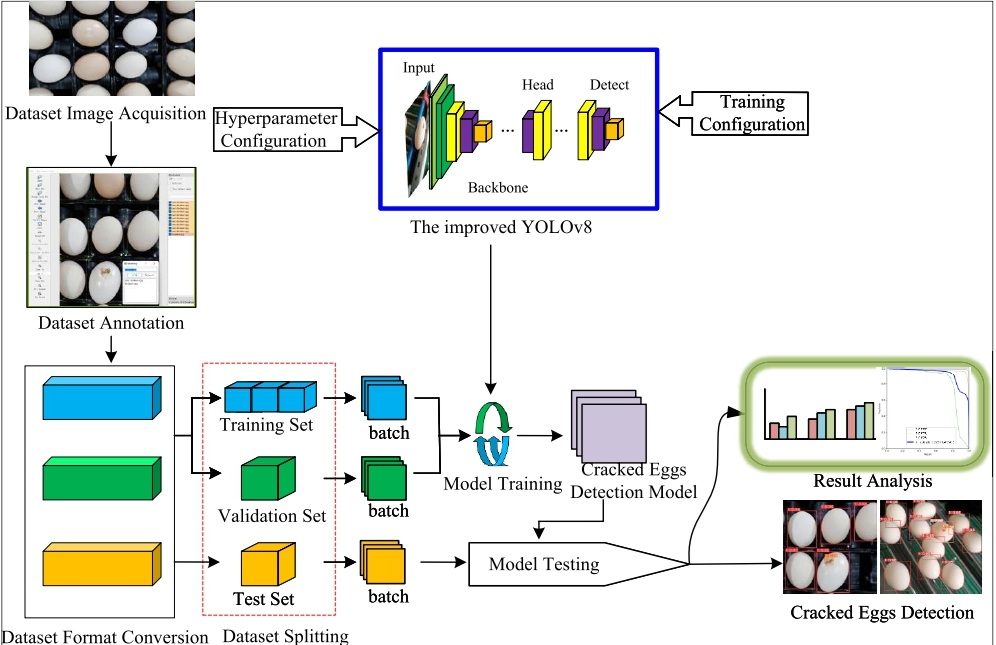
\includegraphics[width=0.9\linewidth,height=0.75\textheight,keepaspectratio]{figure6_training_schematic.jpg}
    \vspace{-0.2cm}
    \caption{\scriptsize Training schematic of the cracked egg detection model (Source: Base Paper Figure 6).}
\end{figure}
\end{frame}

% ==================== SLIDE 21: EVALUATION METRICS ====================
\begin{frame}{Performance Evaluation Metrics}
\textbf{Evaluation Formulas:}
\vspace{-0.15cm}
\begin{equation*}
\text{Precision} = \frac{\text{TP}}{\text{TP} + \text{FP}}, \quad \text{Recall} = \frac{\text{TP}}{\text{TP} + \text{FN}}
\end{equation*}
\vspace{-0.3cm}
\begin{equation*}
\text{FNR} = \frac{\text{FN}}{\text{TP} + \text{FN}}, \quad \text{FPR} = \frac{\text{FP}}{\text{FP} + \text{TN}}
\end{equation*}
\vspace{-0.25cm}
\textbf{Symbol Definitions:}
\vspace{0.12cm}
\begin{itemize}
    \item $\text{TP}$ (True Positives): Defective eggs correctly identified as cracked.
    \item $\text{FP}$ (False Positives): Intact eggs incorrectly flagged as cracked (false alarms).
    \item $\text{TN}$ (True Negatives): Intact eggs correctly identified as intact.
    \item $\text{FN}$ (False Negatives): Cracked eggs incorrectly passed as intact (missed defects).
    \item \textbf{mAP@0.5:} Mean Average Precision across all classes at IoU threshold 0.5.
    \item \textbf{FPS:} Frames Per Second (online real-time threshold $\ge 30$ FPS).
\end{itemize}
\end{frame}

%=====================================================
\section{Results and Performance Analysis}
%=====================================================

% ==================== SLIDE 22: ABLATION STUDY AND COMPLEXITY ====================
\begin{frame}{Ablation Study and Model Complexity}
\begin{table}[h]
\centering
\caption{\scriptsize Ablation experiment results on test dataset (Source: Base Paper Table 1)}
\vspace{-0.3cm}
\setlength{\tabcolsep}{3pt}
\renewcommand{\arraystretch}{0.92}
\resizebox{0.95\textwidth}{!}{
\begin{tabular}{cccc|ccc}
\toprule
\textbf{DCNv2} & \textbf{BiFPN} & \textbf{WIoU} & \textbf{Small Target} & \textbf{Precision (\%)} & \textbf{Recall (\%)} & \textbf{mAP:0.5 (\%)} \\
\midrule
- & - & - & - & 92.2 & 85.3 & 87.7 \\
- & - & \checkmark & - & 90.6 & 87.4 & 90.3 \\
- & \checkmark & - & - & 89.8 & 83.8 & 88.2 \\
- & - & - & \checkmark & 93.8 & 90.3 & 93.0 \\
\checkmark & - & \checkmark & - & 93.1 & 89.4 & 92.1 \\
- & \checkmark & \checkmark & - & 92.6 & 89.5 & 92.2 \\
\checkmark & \checkmark & \checkmark & - & 93.8 & 89.9 & 92.6 \\
\checkmark & \checkmark & \checkmark & \checkmark & \textbf{94.1} & \textbf{90.0} & \textbf{92.9} \\
\bottomrule
\end{tabular}
}
\end{table}
\vspace{-0.35cm}
{\small
\begin{itemize}
    \setlength{\itemsep}{1pt}
    \item Small target head yields the largest single gain (+5.3\% mAP). Full ensemble achieves highest Precision (94.1\%) and balanced robustness.
    \item \textbf{Model Complexity (Table 2):} Parameters: $2.66 \times 10^7$ (+2.7\%), FLOPs: 86.5 G (+9.3\%), Model Size: 51.1 MB (+3.0\%). Significant accuracy boost with minimal overhead.
\end{itemize}
}
\end{frame}

% ==================== SLIDE 23: BENCHMARK COMPARISON ====================
\begin{frame}{Comparative Experiments with Mainstream Detectors}
\begin{table}[h]
\centering
\caption{\scriptsize Comparison across different object detection models (Source: Base Paper Table 3)}
\vspace{-0.3cm}
\setlength{\tabcolsep}{5pt}
\renewcommand{\arraystretch}{0.95}
\resizebox{0.92\textwidth}{!}{
\begin{tabular}{lcccc}
\toprule
\textbf{Model} & \textbf{Precision (\%)} & \textbf{Recall (\%)} & \textbf{mAP:0.5 (\%)} & \textbf{FPS} \\
\midrule
Faster R-CNN (ResNet50) & 68.4 & 80.7 & 78.1 & 17 \\
YOLOv5 & 86.9 & 81.1 & 85.2 & 58 \\
YOLOv8 (Baseline) & 92.2 & 85.3 & 87.7 & 52 \\
YOLOv11 & 92.7 & 84.3 & 87.3 & 47 \\
\textbf{Our Proposed Model} & \textbf{94.1} & \textbf{90.0} & \textbf{92.9} & \textbf{45} \\
\bottomrule
\end{tabular}
}
\end{table}
\vspace{-0.25cm}
{\small
\begin{itemize}
    \setlength{\itemsep}{2pt}
    \item Outperformed Faster R-CNN by 14.8\% mAP despite Faster R-CNN using pretrained weights.
    \item Outperformed recent YOLOv11 by 5.6\% mAP and baseline YOLOv8 by 5.2\% mAP.
    \item At 45 FPS, detection speed easily satisfies production line requirements ($\ge 30$ FPS).
\end{itemize}
}
\end{frame}

% ==================== SLIDE 24: PR CURVES (FULL SLIDE FIGURE 8) ====================
\begin{frame}{Laboratory Testing: Precision-Recall Curves}
\begin{figure}[h]
    \centering
    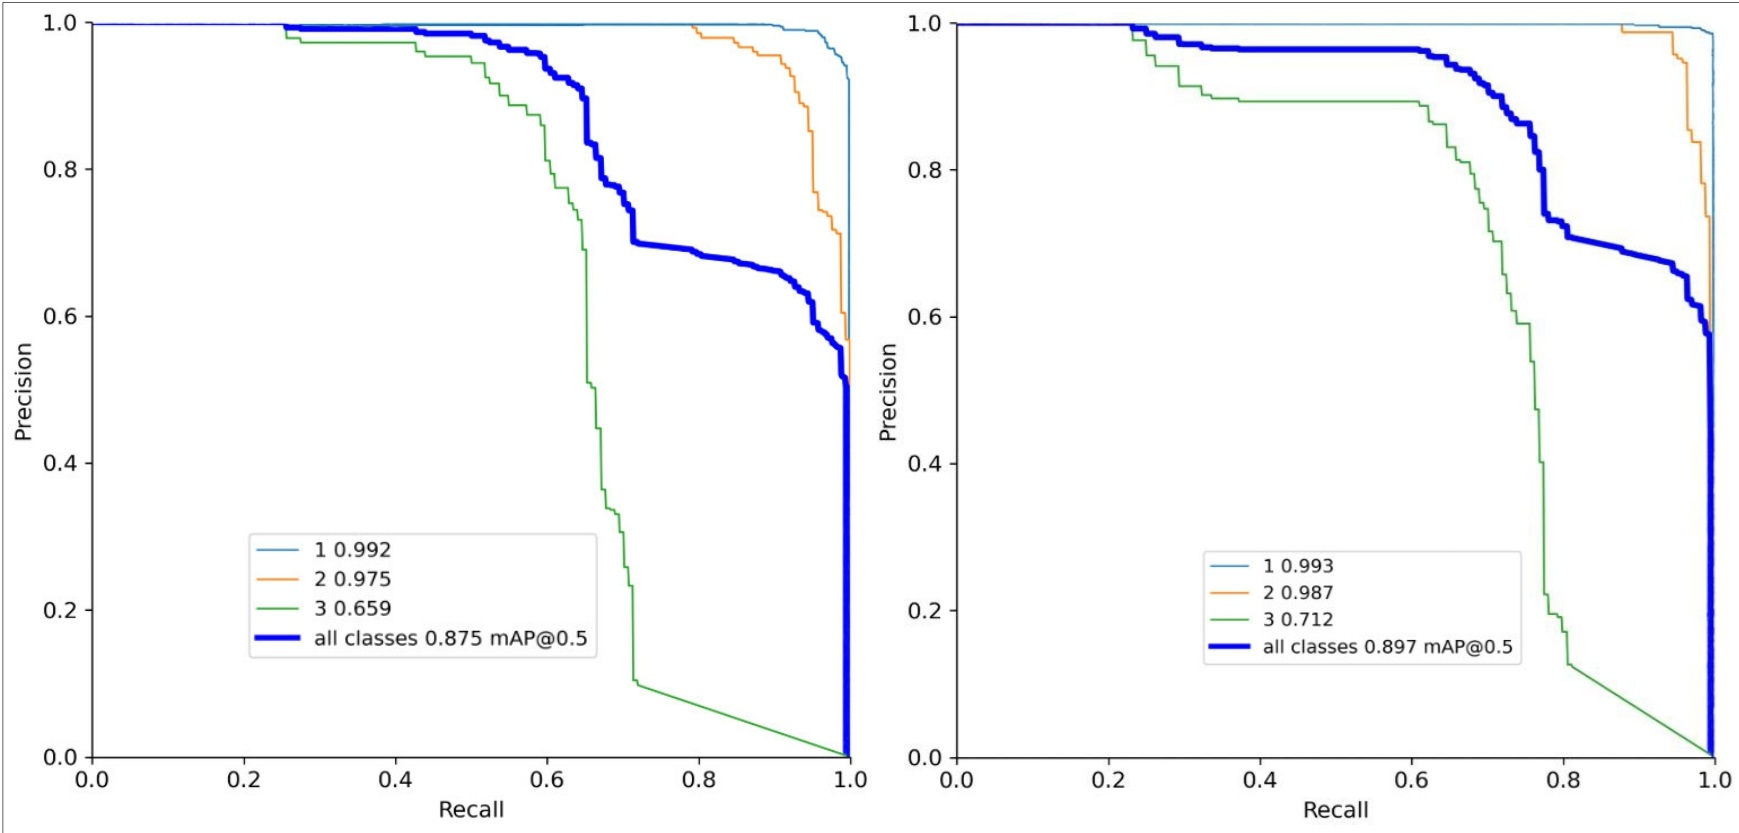
\includegraphics[width=0.88\linewidth,height=0.75\textheight,keepaspectratio]{figure8_pr_curves_comparison.jpg}
    \vspace{-0.2cm}
    \caption{\scriptsize Precision-Recall curves before and after model improvement (Source: Base Paper Figure 8).}
\end{figure}
\end{frame}

% ==================== SLIDE 25: VISUAL DETECTION (FULL SLIDE FIGURE 9) ====================
\begin{frame}{Laboratory Testing: Visual Detection Comparison}
\begin{figure}[h]
    \centering
    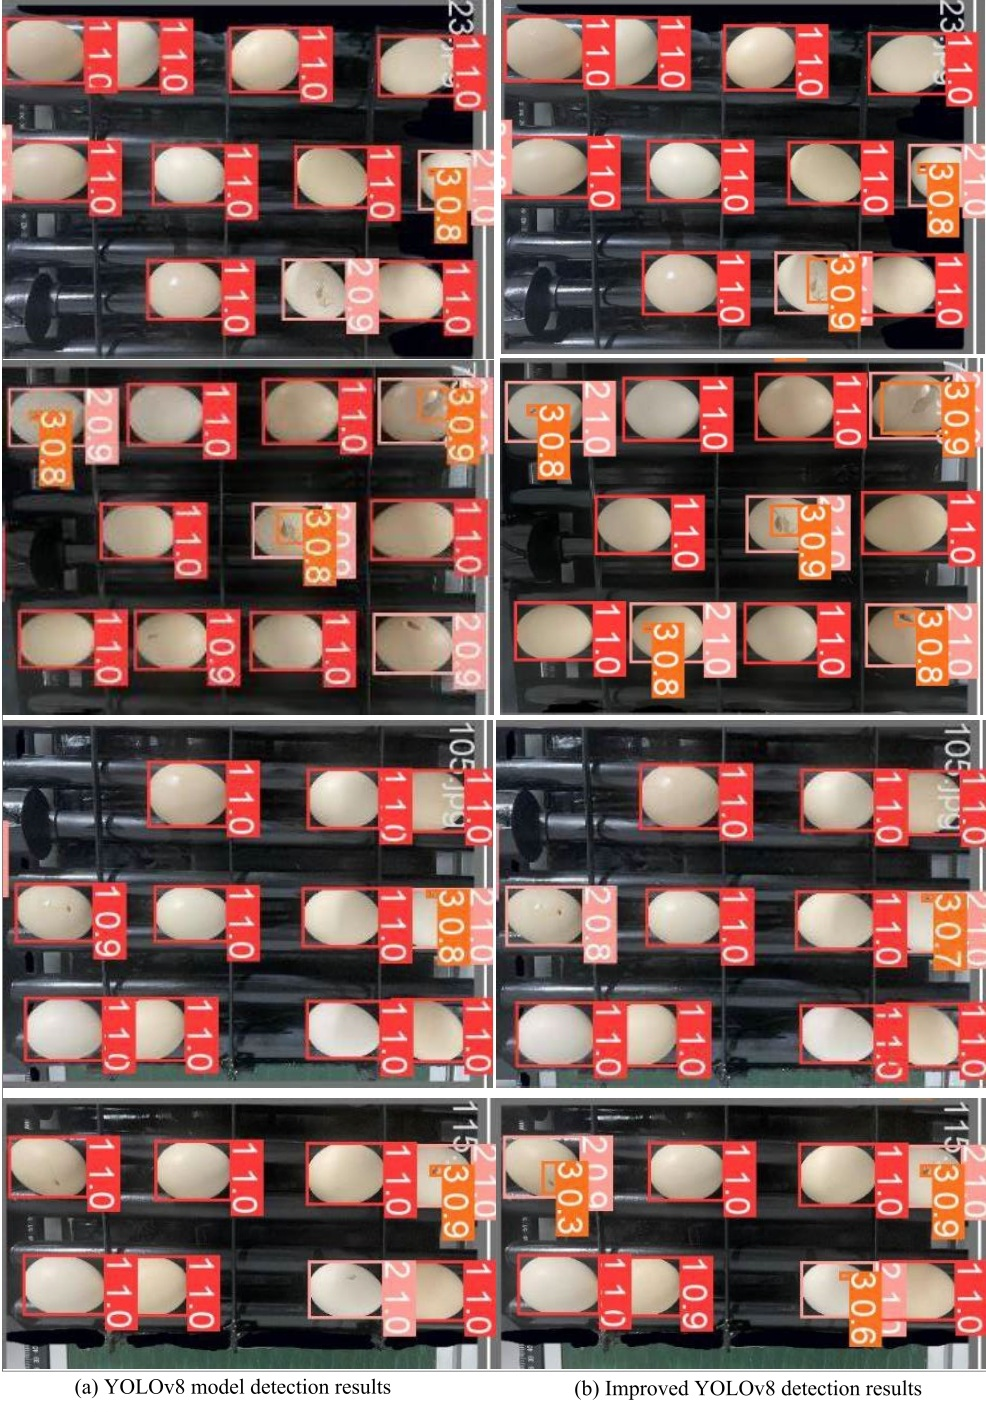
\includegraphics[width=0.88\linewidth,height=0.75\textheight,keepaspectratio]{figure9_detection_effects_comparison.jpg}
    \vspace{-0.2cm}
    \caption{\scriptsize Visual detection comparison on test frames (Source: Base Paper Figure 9). Left: YOLOv8. Right: Improved YOLOv8.}
\end{figure}
\end{frame}

%=====================================================
\section{Industrial Deployment and Factory Testing}
%=====================================================

% ==================== SLIDE 26: FACTORY DEPLOYMENT (FULL SLIDE FIGURE 7) ====================
\begin{frame}{Industrial Deployment Workflow and Equipment}
\begin{figure}[h]
    \centering
    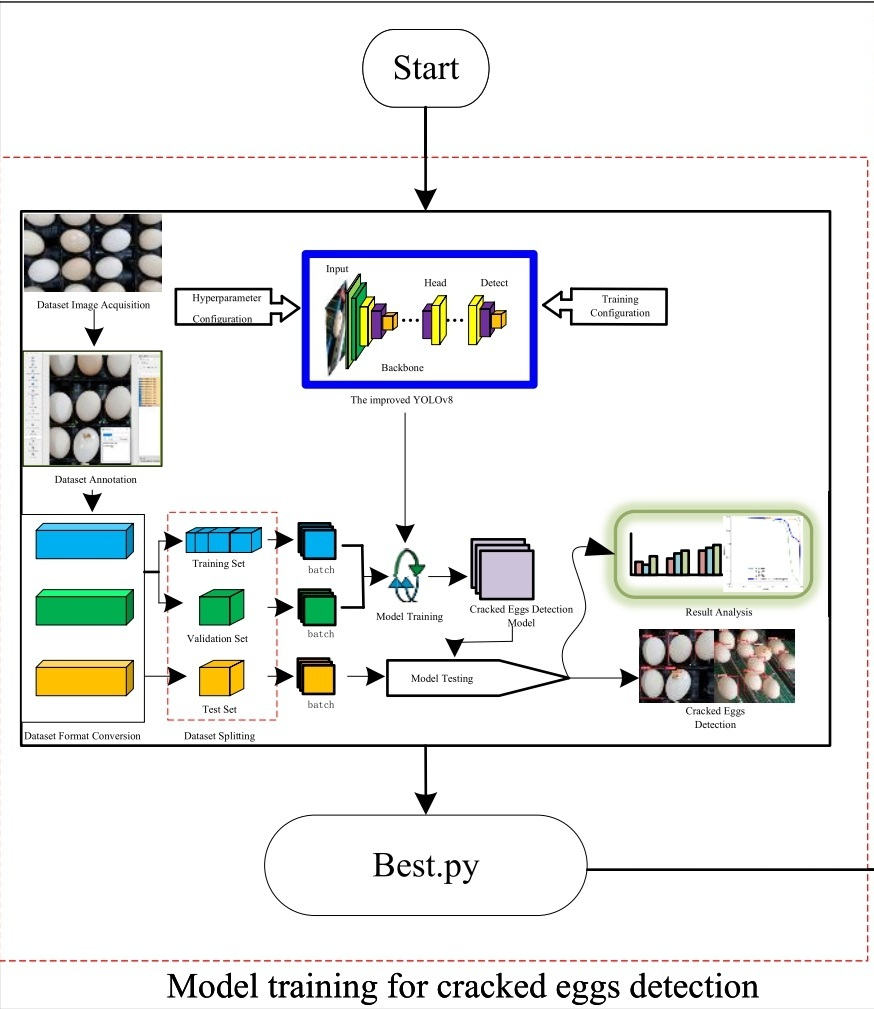
\includegraphics[width=0.85\linewidth,height=0.36\textheight,keepaspectratio]{figure7_online_deployment_testing_1.jpg} \\
    \vspace{0.1cm}
    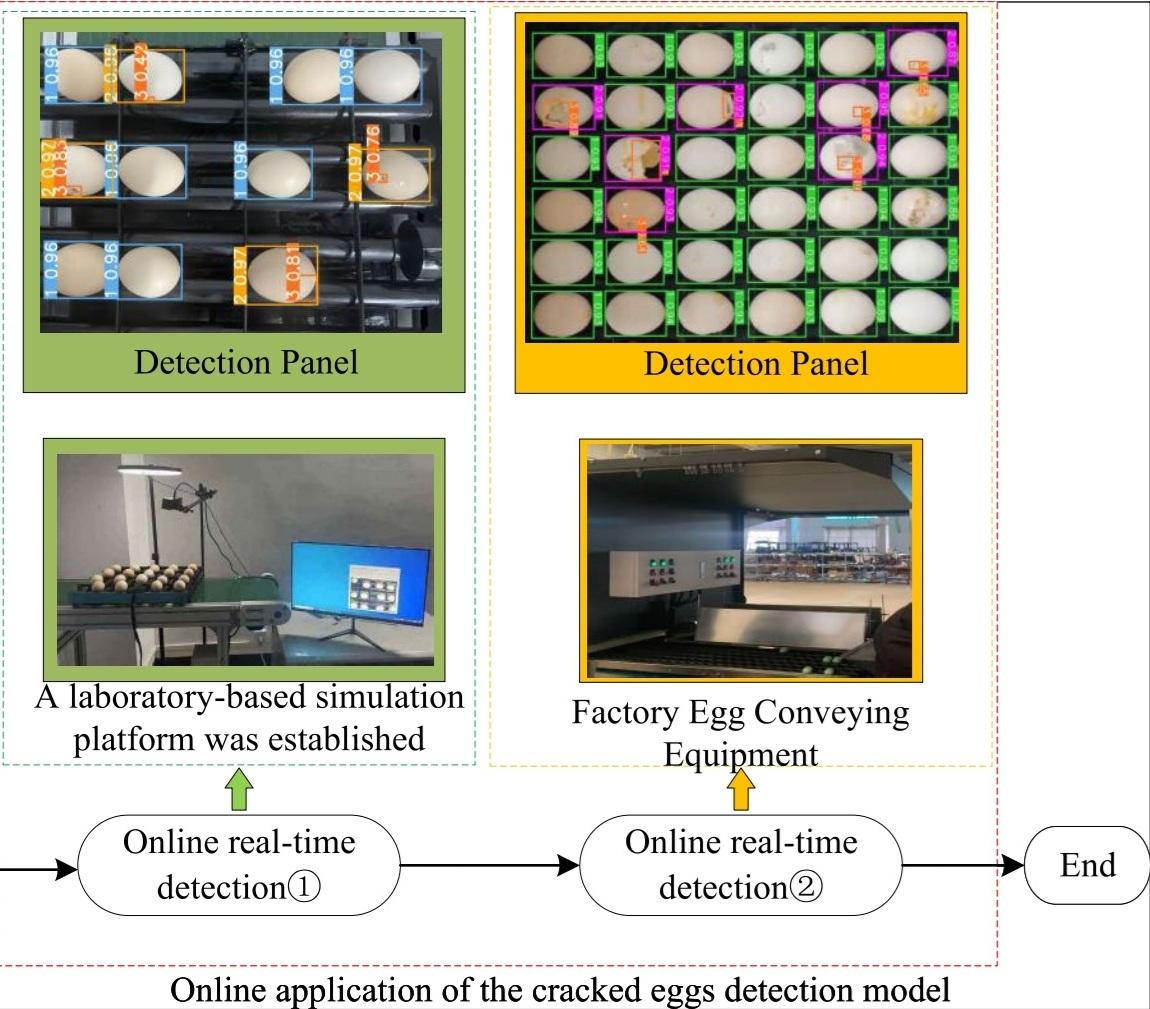
\includegraphics[width=0.85\linewidth,height=0.36\textheight,keepaspectratio]{figure7_online_deployment_testing_2.jpg}
    \vspace{-0.2cm}
    \caption{\scriptsize Online deployment testing on factory equipment (Source: Base Paper Figure 7).}
\end{figure}
\end{frame}

% ==================== SLIDE 27: FACTORY ACCURACY ====================
\begin{frame}{Factory Online Inspection Accuracy (FNR and FPR)}
\begin{table}[h]
\centering
\caption{\scriptsize Online inspection comparison on 106 production frames (Source: Base Paper Tables 5 and 6)}
\vspace{-0.3cm}
\setlength{\tabcolsep}{3.5pt}
\renewcommand{\arraystretch}{0.92}
\resizebox{0.95\textwidth}{!}{
\begin{tabular}{l|cc|cc}
\toprule
\textbf{Category} & \multicolumn{2}{c|}{\textbf{Baseline YOLOv8}} & \multicolumn{2}{c}{\textbf{Proposed Improved YOLOv8}} \\
& \textbf{FNR (\%)} & \textbf{FPR (\%)} & \textbf{FNR (\%)} & \textbf{FPR (\%)} \\
\midrule
Class 1: Intact Egg & 1.26 & 4.00 & \textbf{0.46} & \textbf{2.18} \\
Class 2: Cracked Egg & 10.17 & 3.20 & \textbf{5.52} & \textbf{1.16} \\
Class 3: Damaged Area & 22.97 & 0.87 & \textbf{19.19} & \textbf{0.58} \\
\midrule
\textbf{Compound Dual Verification FNR} & \multicolumn{2}{c|}{$10.17\% \times 22.97\% = 2.34\%$} & \multicolumn{2}{c}{$\mathbf{5.52\% \times 19.19\% = 1.06\%}$} \\
\bottomrule
\end{tabular}
}
\end{table}
\vspace{-0.3cm}
{\small
\begin{itemize}
    \setlength{\itemsep}{1pt}
    \item False alarm rate for intact eggs dropped from 4.00\% to 2.18\%, saving intact eggs.
    \item Compound miss rate for cracked eggs fell to 1.06\%, reliably filtering defective eggs.
\end{itemize}
}
\end{frame}

% ==================== SLIDE 28: PRODUCTION LINE DETECTIONS (FULL SLIDE FIGURE 10) ====================
\begin{frame}{Production Line: Visual Detection Results}
\begin{figure}[h]
    \centering
    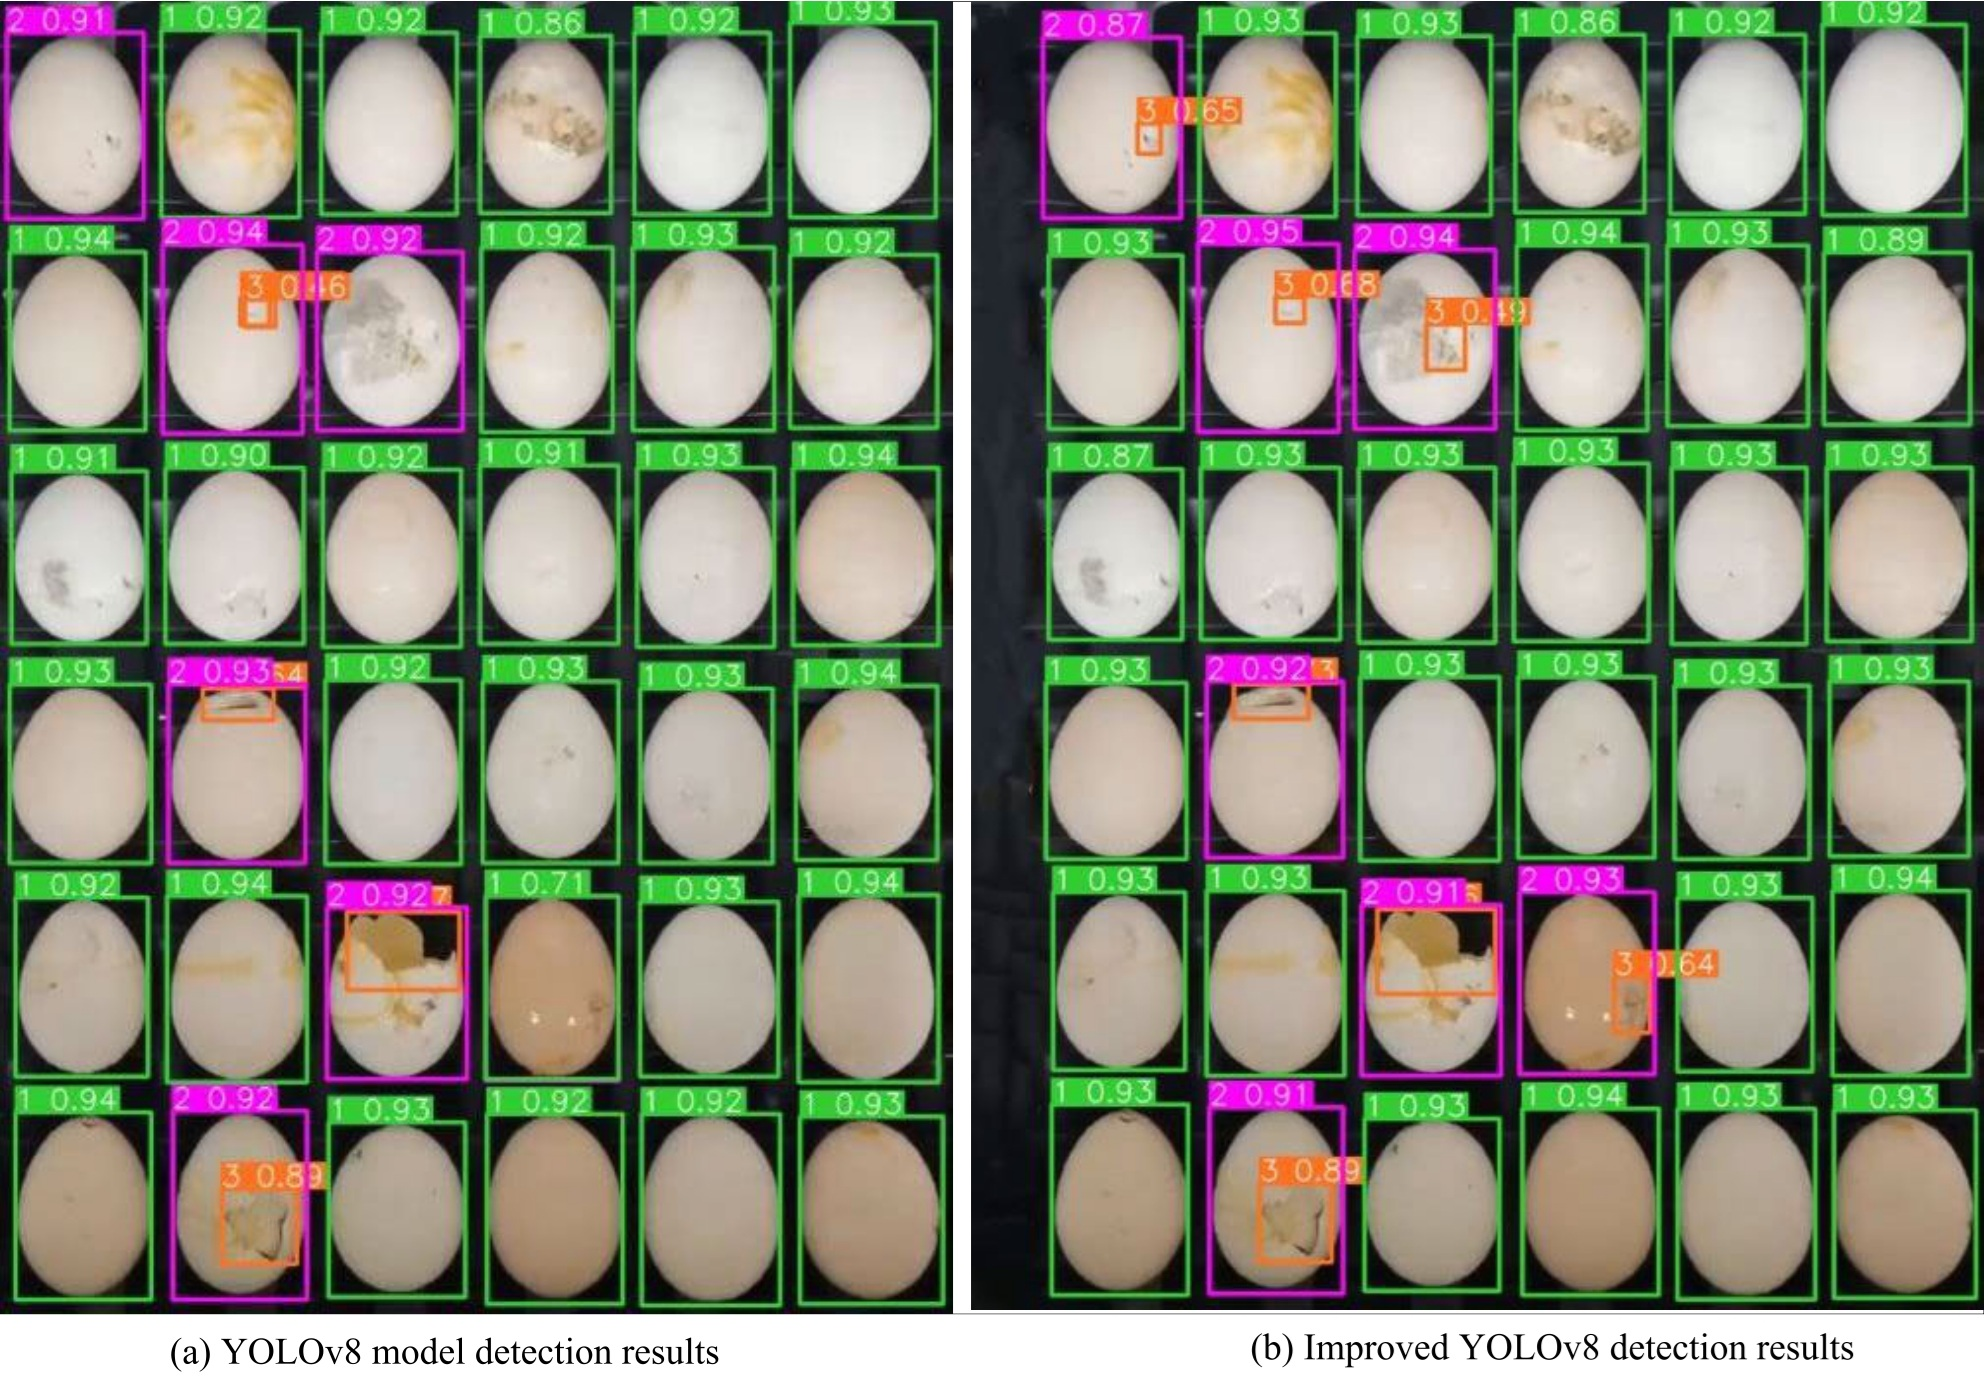
\includegraphics[width=0.88\linewidth,height=0.75\textheight,keepaspectratio]{figure10_production_line_detection.jpg}
    \vspace{-0.2cm}
    \caption{\scriptsize Detection effect on actual production line (Source: Base Paper Figure 10). Green: Intact, Purple: Cracked, Brown: Damaged Area.}
\end{figure}
\end{frame}

% ==================== SLIDE 29: SPEED STABILITY (FULL SLIDE FIGURE 11) ====================
\begin{frame}{Production Line: Detection Speed Stability}
\begin{figure}[h]
    \centering
    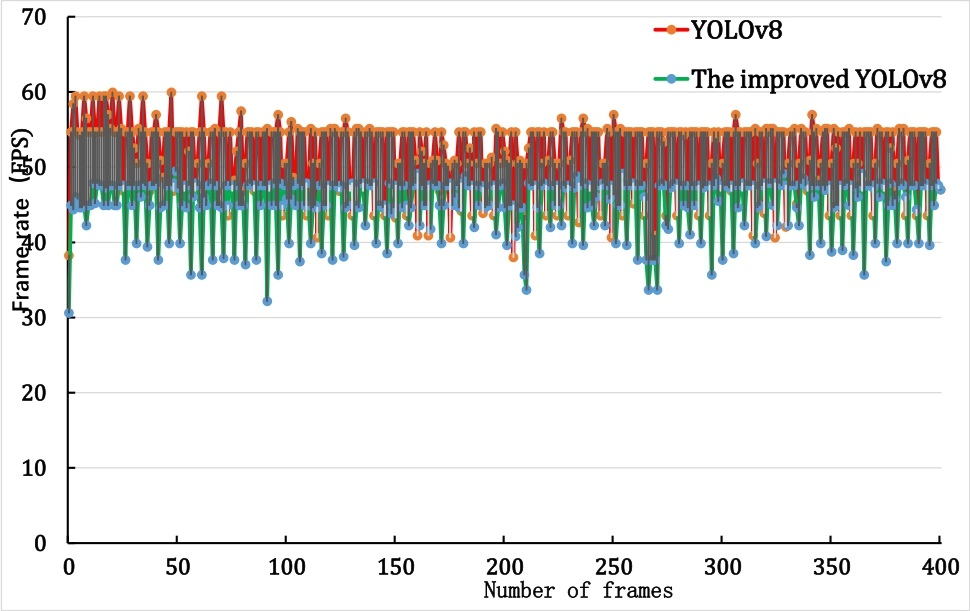
\includegraphics[width=0.88\linewidth,height=0.75\textheight,keepaspectratio]{figure11_online_detection_speed.jpg}
    \vspace{-0.2cm}
    \caption{\scriptsize Online detection frame rate stability across 400 frames (Source: Base Paper Figure 11).}
\end{figure}
\end{frame}

%=====================================================
\section{Discussion and Conclusion}
%=====================================================

% ==================== SLIDE 30: DISCUSSION ====================
\begin{frame}{Discussion: Operational Findings and Edge Cases}
\small
\begin{itemize}
    \item \textbf{Speed vs Accuracy Trade-off:} 14.5\% speed reduction (52 to 45 FPS) gives a +5.2\% mAP boost; 45 FPS well exceeds factory line demands ($\ge 30$ FPS).
    \medskip
    \item \textbf{Surface Adaptability:} Demonstrated high detection reliability on both unwashed farm eggs and pre-washed supermarket eggs.
    \medskip
    \item \textbf{Eggshell Varieties:} Solid shells (duck eggs) show high contrast; patterned shells (quail eggs) create background interference.
    \medskip
    \item \textbf{Reticular Micro-Cracks:} Fine net-like cracks possess low pixel areas and weak gradients, posing the primary challenge for future work.
\end{itemize}
\end{frame}

% ==================== SLIDE 31: CONCLUSION AND FUTURE SCOPE ====================
\begin{frame}{Conclusion and Future Scope}
\small
\textbf{Conclusion:}
\begin{itemize}
    \item Developed a real-time detection system combining rotational conveyance, improved YOLOv8 and dual verification.
    \item Integrated DCNv2, BiFPN, WIoUv2 and a P2 small target head, achieving 92.9\% mAP and 45 FPS.
    \item Lowered compound broken egg miss rate to 1.06\% on factory equipment, meeting industrial inspection criteria.
\end{itemize}
\bigskip
\textbf{Future Scope:}
\begin{itemize}
    \item Adopt dark-box illumination setups to enhance contrast for faint net-like hairline cracks.
    \item Explore super-resolution and attention-guided magnification for micro-defects.
    \item Expand datasets to diverse poultry species and integrate internal defect detection (scattered yolk, blood spots).
\end{itemize}
\end{frame}

% ==================== SLIDE 32: REFERENCES PART 1 ====================
\begin{frame}{References: Foundational and Survey Literature}
\scriptsize
\begin{thebibliography}{5}
\bibitem[1]{sun2026} D. Sun, H. Wei, Y. Luo, W. Li and Y. Yu, ``Real-Time Detection Method for Cracked Eggs Based on Improved YOLOv8 and Dual Verification With Triple Classification Granularity,'' \textit{IEEE Access}, vol. 14, pp. 62322-62333, 2026.
\bibitem[2]{liang2020} D. Liang, P. Li, D. Liang, J. Qian and B. Li, ``Integrated detection and grading system for internal and external quality of eggs based on machine vision,'' \textit{J. Chin. Inst. Food Sci. Technol.}, vol. 20, no. 11, pp. 247-254, 2020.
\bibitem[3]{datta2019} A. Datta, B. Botta and S. Gattam, ``Damage detection on chicken eggshells using faster R-CNN,'' in \textit{Proc. ASABE Annu. Int. Meeting}, 2019, p. 1244.
\bibitem[4]{turkoglu2021} M. Turkoglu, ``Defective egg detection based on deep features and bidirectional long-short-term-memory,'' \textit{Comput. Electron. Agricult.}, vol. 185, Jun. 2021, Art. no. 106152.
\bibitem[5]{botta2022} B. Botta, S. S. R. Gattam and A. K. Datta, ``Eggshell crack detection using deep convolutional neural networks,'' \textit{J. Food Eng.}, vol. 315, Feb. 2022, Art. no. 110798.
\end{thebibliography}
\end{frame}

% ==================== SLIDE 33: REFERENCES PART 2 ====================
\begin{frame}{References: YOLO Adaptations and Architectures}
\scriptsize
\begin{thebibliography}{5}
\bibitem[6]{yin2024} J. Yin, J. Kang and D. Xiao, ``Lightweight duck egg crack detection algorithm based on improved YOLOv5l,'' \textit{Trans. Chin. Soc. Agricult. Eng.}, vol. 40, no. 1, pp. 165-173, 2024.
\bibitem[7]{huang2023} Y. Huang, Y. Luo, Y. Cao, X. Lin, H. Wei, M. Wu, X. Yang and Z. Zhao, ``Damage detection of unwashed eggs through video and deep learning,'' \textit{Foods}, vol. 12, no. 11, p. 2179, 2023.
\bibitem[8]{zhu2019} X. Zhu, H. Hu, S. Lin and J. Dai, ``Deformable ConvNets v2: More Deformable, Better Results,'' in \textit{Proc. IEEE/CVF CVPR}, 2019, pp. 9308-9316.
\bibitem[9]{tan2020} M. Tan, R. Pang and Q. V. Le, ``EfficientDet: Scalable and Efficient Object Detection,'' in \textit{Proc. IEEE/CVF CVPR}, 2020, pp. 10778-10787.
\bibitem[10]{tong2023} Z. Tong, Y. Chen, Z. Xu and R. Yu, ``Wise-IoU: Bounding Box Regression Loss with Dynamic Focusing Mechanism,'' \textit{arXiv preprint arXiv:2301.10051}, 2023.
\end{thebibliography}
\end{frame}

% ==================== SLIDE 34: FINAL SLIDE ====================
\begin{frame}
\centering
\Huge \textbf{Thank You!} \\
\bigskip
\Large Questions and Discussion
\end{frame}

\end{document}